\documentclass[tikz]{standalone}
\usepackage{pgfplots}
\pgfplotsset{compat=1.15}
\usepackage{mathrsfs}
\usetikzlibrary{arrows,calc}
\usepackage{tkz-euclide}

\usepackage{fp}
\pagestyle{empty}

\definecolor{AngleClr}{rgb}{0,0.39215686274509803,0}
\definecolor{ShapeClr}{rgb}{0.6,0.2,0}
\definecolor{BlueClr}{RGB}{5,81,163}
\definecolor{RedClr}{RGB}{199, 28, 16}
\definecolor{YellowClr}{RGB}{191, 159, 0}

\newcommand\encircle[1]{%
  \tikz[baseline=(X.base)] 
    \node (X) [draw,fill=white,shape=circle, inner sep=0] {\strut #1};}

\begin{document}

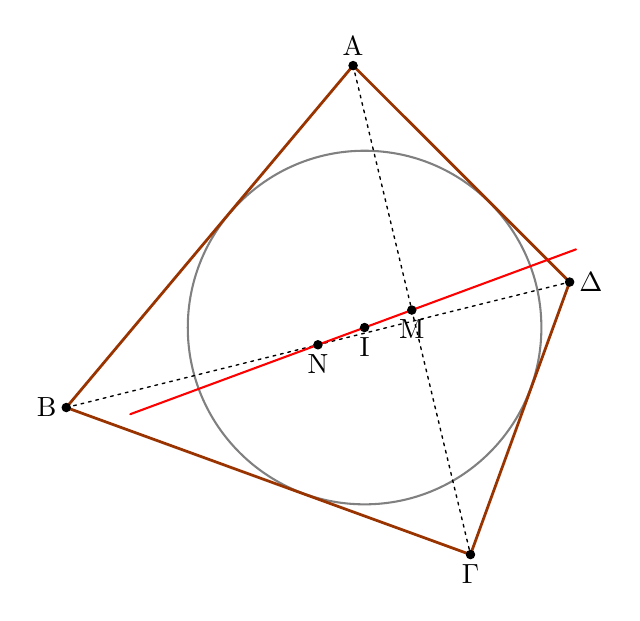
\begin{tikzpicture}[scale=.75]
\tkzSetUpLine[line width=1pt,color=black]
\tkzSetUpPoint[fill=black]

\tkzDefPoints{0/0/I}

% Define the points where the circle touches the quadrilateral.
\tkzDefPoint(45:3){Id}
\tkzDefPoint(-20:3){Ic}
\tkzDefPoint(-110:3){Ib}
\tkzDefPoint(140:3){Ia}

% Find the lines containing the sides of the quadrilateral.
\tkzDefLine[tangent at=Ia](I) \tkzGetPoint{h1}
\tkzDefLine[tangent at=Ib](I) \tkzGetPoint{h2}
\tkzDefLine[tangent at=Ic](I) \tkzGetPoint{h3}
\tkzDefLine[tangent at=Id](I) \tkzGetPoint{h4}


% Find the vertices of the quadrilateral.
\tkzInterLL(Id,h4)(Ia,h1)\tkzGetPoint{A}
\tkzInterLL(Ia,h1)(Ib,h2)\tkzGetPoint{B}
\tkzInterLL(Ib,h2)(Ic,h3)\tkzGetPoint{C}
\tkzInterLL(Ic,h3)(Id,h4)\tkzGetPoint{D}

\tkzFillPolygon[fill=white](A,B,C,D)


\tkzDefMidPoint(A,C) \tkzGetPoint{M}
\tkzDefMidPoint(B,D) \tkzGetPoint{N}

\tkzDrawCircle[line width=0.75](I,Ia)

% Draw the quadrilateral.

\tkzDrawPolygon[color=ShapeClr](A,B,C,D)

\tkzDrawSegments[line width=0.5pt,color=black,dashed,dash pattern=on 1pt off 1.75pt](A,C B,D)

\tkzDrawSegment[line width=0.75pt,color=red,add=1.75 and 2](M,N)


% \tkzDrawSegments[line width=1pt,color=ShapeClr]()

\tkzDrawPoints[size=3](A,B,C,D,M,N,I)

\tkzLabelPoint[below](I){$\rm I$}
\tkzLabelPoint[below](M){$\rm M$}
\tkzLabelPoint[below](N){$\rm N$}



\tkzLabelPoint[above](A){$\rm A$}
\tkzLabelPoint[left](B){$\rm B$}
\tkzLabelPoint[below](C){$\rm \Gamma$}
\tkzLabelPoint[right](D){$\rm \Delta$}

\end{tikzpicture}

\end{document}
